\documentclass{article}

\usepackage{graphicx}
\usepackage{tikz}
\usepackage{tikzsymbols}
\usetikzlibrary{calc,patterns,shapes.geometric}
\pagestyle{empty}

\def\centerarc[#1](#2)(#3:#4:#5){\draw[#1] ($(#2)+({#5*cos(#3)},{#5*sin(#3)})$) arc (#3:#4:#5);}

\begin{document}
	\centering
	\begin{figure}
			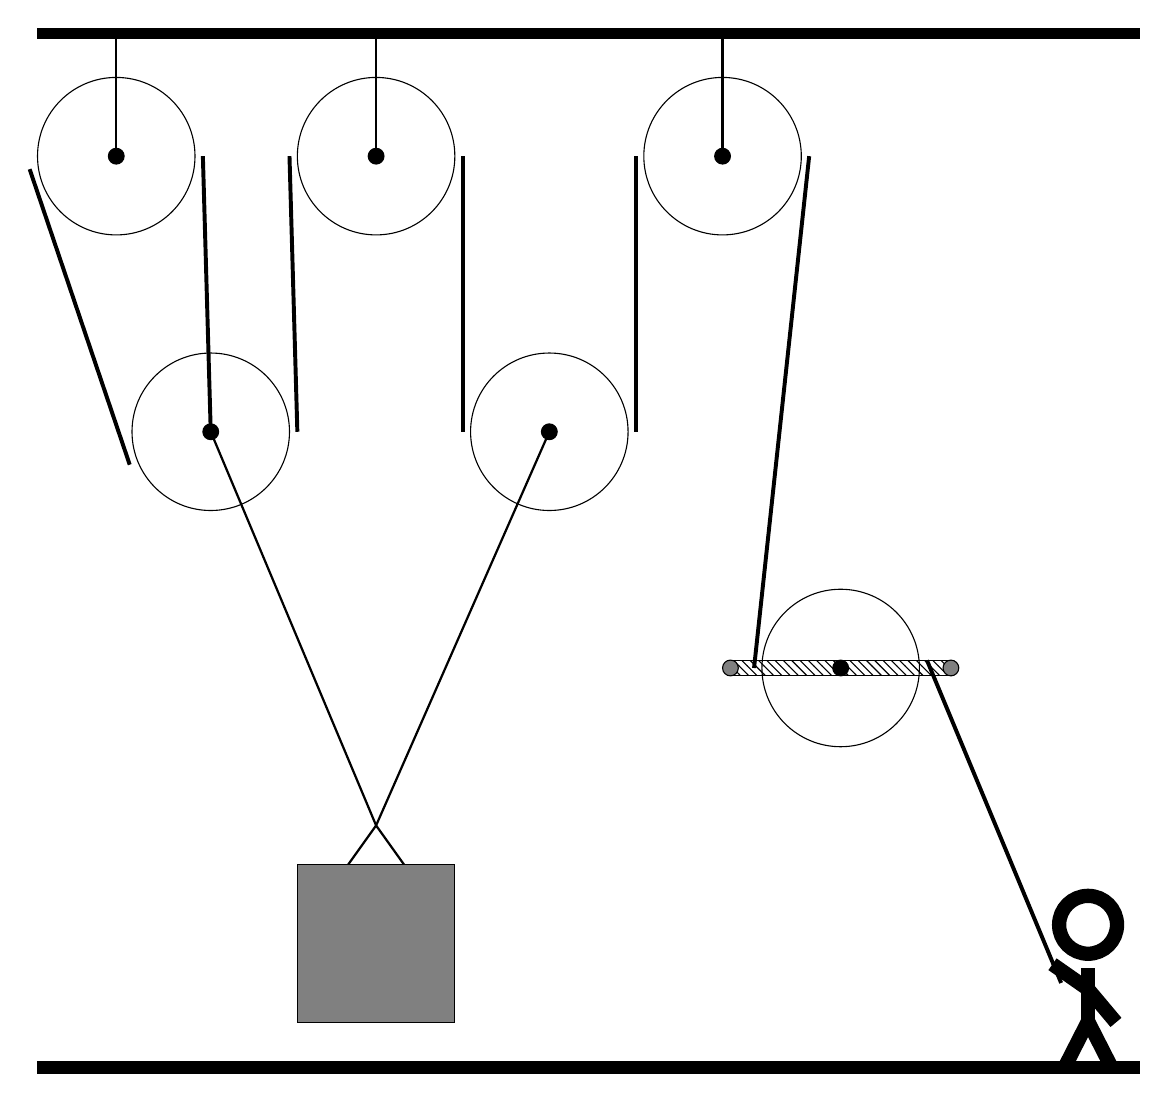
\begin{tikzpicture}
				%%%%% START %%%%%
								\draw[fill=black] (-2, 10) rectangle (12, 10.125);
				
				\draw (-1, 8.5) circle (1);
				\draw[fill=black] (-1, 8.5) circle (0.1);
				\draw[thick] (-1, 8.5) -- (-1, 10);
				
				\draw (2.3, 8.5) circle (1);
				\draw[fill=black] (2.3, 8.5) circle (0.1);
				\draw[thick] (2.3, 8.5) -- (2.3, 10);
				
				\draw (6.7, 8.5) circle (1);
				\draw[fill=black] (6.7, 8.5) circle (0.1);
				\draw[thick] (6.7, 8.5) -- (6.7, 10);
				
				\draw (0.2, 5) circle (1);
				\draw[fill=black] (0.2, 5) circle (0.1);
				
				\draw (4.5, 5) circle (1);
				\draw[fill=black] (4.5, 5) circle (0.1);
				
				\draw (8.2, 2) circle (1);
				\draw[fill=black] (8.2, 2) circle (0.1);
				\draw[pattern=north west lines, pattern color=black] (6.8, 2.1) rectangle (9.6, 1.9);
				\draw[fill=black!50] (6.8, 2) circle (0.1);
				\draw[fill=black!50] (9.6, 2) circle (0.1);
				
				\draw[thick] (0.2, 5) -- (2.3, 0)  -- (4.5, 5);
				\draw[thick]  (1.8, -0.7) -- (2.3, 0) -- (2.8, -0.7);
				\draw[fill=black!50] (1.3, -0.5) rectangle (3.3, -2.5);
				
				\draw[line width=0.5mm] (0.2, 5) -- (0.1, 8.5);
				\centerarc[line width=0.5mm](-1, 8.5)(0:200:1.1);
				\draw[line width=0.5mm] (-2.1, 8.335) -- (-0.829, 4.582);
				\centerarc[line width=0.5mm](0.2, 5)(200:360:1.1);
				\draw[line width=0.5mm](1.3, 5) -- (1.2, 8.5);
				\centerarc[line width=0.5mm](2.3, 8.5)(0:180:1.1);
				\draw[line width=0.5mm] (3.4, 8.5) -- (3.4, 5);
				\centerarc[line width=0.5mm](4.5, 5)(180:360:1.1);
				\draw[line width=0.5mm] (5.6, 5) -- (5.6, 8.5);
				\centerarc[line width=0.5mm](6.7, 8.5)(0:180:1.1);
				\draw[line width=0.5mm](7.8, 8.5) --  (7.1, 2);
				\centerarc[line width=0.5mm](8.2, 2)(180:220:1.1);
				\draw[line width=0.5mm](9.296, 2.097) -- (11, -2);
				
				\node at (11.3, -2) {\Strichmaxerl[10][-35][-50]};
				
				\draw[fill=black] (-2, -3) rectangle (12, -3.15);
				%%%%% END %%%%%
			\end{tikzpicture}
	\end{figure}	
\end{document}